\documentclass[11pt, oneside]{report}
\usepackage[a4paper,top=3cm,bottom=3cm,left=3cm,right=2cm]{geometry}
\usepackage[utf8]{inputenc}
\usepackage[T1]{fontenc}
\usepackage{graphicx}
\usepackage{url}
\usepackage{float}
\usepackage{titlesec}
\usepackage{pdfpages}
\usepackage{lmodern}

\usepackage[hidelinks,breaklinks]{hyperref}
\usepackage[slovak]{babel} % vypnite pre prace v anglictine
\usepackage{listings}
\usepackage{graphicx}
\usepackage{chngcntr}
\counterwithout{equation}{chapter}
\graphicspath{ {images/} }

\usepackage{color}
\definecolor{gray}{rgb}{0.4,0.4,0.4}
\definecolor{darkblue}{rgb}{0.0,0.0,0.6}
\definecolor{cyan}{rgb}{0.0,0.6,0.6}
\definecolor{orange}{rgb}{1,0.45,0}

%\lstset{
 % basicstyle=\ttfamily,
  %columns=fullflexible,
  %showstringspaces=false,
  %commentstyle=\color{gray}\upshape
%}
\lstset
{
basicstyle=\ttfamily,
keywordstyle=\color{blue},
identifierstyle=\color[RGB]{43,145,175},
commentstyle=\slshape\color[RGB]{0,128,0},
stringstyle=\color[RGB]{163,21,21},
breaklines=true,
tabsize=3,
columns=fullflexible,
showstringspaces=false,
frame=lines,
captionpos=b
}

\lstdefinelanguage{XML}
{
  morestring=[b]",
  morestring=[s]{>}{<},
  morecomment=[s]{<?}{?>},
  stringstyle=\color{black},
  identifierstyle=\color{darkblue},
  keywordstyle=\color{cyan},
  morekeywords={xmlns,version,type}% list your attributes here
}

\lstdefinelanguage{JavaScript}{
  morekeywords={typeof, new, true, false, catch, function, return, null, catch, switch, var, if, in, while, do, else, case, break, this, async, public, Task, private, String, string, implements, export, class, let, any, static, throw, constructor, console, change, ngModel, <mat-select, mat-option , ngFor, jQuery, parseXML, await, get, set, TimeSpan },
  morecomment=[s]{/*}{*/},
  morecomment=[l]//,
  morestring=[b]",
  morestring=[b]'
}

\lstdefinelanguage{HTML5}{
		showstringspaces=true,
		keepspaces=true,
        language=html,
        sensitive=true, 
		literate=%
		{@}{{{\color{orange}@}}}1
		{\{}{{{\color{orange}\{}}}1
		{\}}{{{\color{orange}\}}}}1,
        alsoletter={<>=-},
        otherkeywords={
        % HTML tags
        <html>, <head>, <title>, </title>, <meta, />, </head>, <body>,
        <canvas, \/canvas>, <script>, </script>, </body>, </html>, <!, html>, <style>, </style>, ><
        },
        ndkeywords={
        % General
        =,
        % HTML attributes
        charset=, id=, width=, height=,display, display:
        % CSS properties
        border:, transform:, -moz-transform:, transition-duration:, transition-property:, transition-timing-function:
        },  
        morecomment=[s]{<!--}{-->},
        tag=[s],        
}

\usepackage[backend=bibtex,
                style=authoryear,
                natbib=true, 
                style=numeric-comp
                ]{biblatex} 
\DeclareFieldFormat{url}{\url{#1}}
\bibliography{literatura.bib} 
\linespread{1.2} % hodnota 1.25 by mala zodpovedat 1.5 riadkovaniu
\pagenumbering{arabic} 
\urlstyle{same}

\titleformat{\chapter}{\normalfont\huge\bf}{\thechapter.}{20pt}{\bf}
\titlespacing*{\chapter}{0pt}{0pt}{20pt}

% -----------------
% --- Definicia zakladnych pojmov
% --- Vyplnte podla vasho zadania
% -------------------
\def\mfrok{2018}
\def\mfnazov{BAKALÁRSKA PRÁCA}
\def\mfnazovprace{Absolvovanie individuálnej odbornej praxe\\
Individual Professional Practice in the
Company
}
\def\mfautor{Michal Falát}
\def\mfskolitel{Petr Šaloun }
\def\mfkonzultant{Boros Kovař }  

\def\mfmiesto{Ostrava, \mfrok}
\def\mfodbor{2508 Informatika} 
\def\program{ Informatika }
\def\mfpracovisko{ Katedra informatiky }
\def\mftyp{bakalarka }
\renewcommand{\lstlistingname}{Výpis}
\renewcommand{\lstlistlistingname}{Zoznam výpisov zdrojového kódu}
\begin{document}  


% -------------------
% --- Obalka ------
% -------------------
\thispagestyle{empty}

\begin{center}
\sc\large
VŠB - Technická univerzita Ostrava\\
Fakulta elektrotechniky a informatiky


\vfill

{\LARGE\mfnazov}\\
\end{center}

\vfill

{\sc\large 
\noindent \mfrok \hfill  \hfill \mfautor
}

\eject % EOP i
% --- koniec obalky ----


\thispagestyle{empty}
\noindent
\begin{center}
{\LARGE
V\v SB - Technická univerzita Ostrava\\
Fakulta elektrotechniky a informatiky\\
Katedra informatiky\\}

\vfill

{\huge\textbf\mfnazovprace}\\
\end{center}

\vfill



{\LARGE
\noindent \mfrok \hfill  \hfill \mfautor
}

\eject % EOP i

%\newpage
%
\includepdf[pages={1}]{zadanie.pdf}
\newpage 

\includepdf[pages={1}]{vyhlasenie.pdf}
%\vspace*{\fill}
%Prehlasujem, že som túto bakalársku prácu vypracoval samostatne. Uviedol som všetky literárne pramene a publikácie, z ktorých som čerpal.\\\\\\
%V Ostrave 25. apríla \hfill .........................................

\newpage 
\thispagestyle{empty}

\vspace*{\fill}
{\bf Poďakovanie:} Chcel by som poďakovať svojim kolegom  z práce, ktorí si na mňa našli čas a boli ochotní mi pomôcť a vysvetliť akýkoľvek problém. Poďakovanie patrí aj môjmu konzultantovi, Borisovi, ktorý mi zastrešil odbornú prax a venoval mi aj svoj voľný čas.


% --- Koniec poďakovania

% -------------------
%   Abstrakt - Slovensky
% -------------------
\newpage
\thispagestyle{empty}
\section*{Abstrakt}


Táto bakalárska práca popisuje absolvovanie odbornej praxe vo firme M2M Solutions. V prvej časti je v krátkosti   vysvetlená činnosť a hlavné zameranie firmy, ale aj moje pracovné zaradenie. V ďalšej kapitole  v krátkosti popisujem  hlavné technológie, s ktorými som sa počas praxe najviac stretával. Ďalšia  kapitola je venovaná samotným projektom a zadaným úlohám,  spolu s~riešeniami, na ktorých som  počas obidvoch semestrov pracoval. Pomedzi úlohy sú v vysvetlené aj konkrétne  časti technologii ale aj problematika, ktorú riešia. V závere práce popisujem  celkový súhrn  a využitie  znalostí  nadobudnutých počas školy a technológie, ktoré  som sa musel individuálne doučiť.



\paragraph*{Kľúčové slová:} ASP.NET, C\#, Java, Angular, Typescript, MVC
% --- Koniec Abstrakt - Slovensky

\paragraph*{}

\section*{Abstract}
This bachelor thesis describes my individual practise in company M2M Solutions. In the first section I explain the company's  activities and main focus. In the next section I describe basic theory about technologies, which I most used. Next section is dedicated to projects and tasks with solutions, which I work on during practise. Between tasks are briefly explained  parts of~technologies, which  I used and problematics, which they deal with. Finally, I explain total summary of practise and usage of technologies, that a learnt during school and technologies which I have to learn on my own.


\paragraph*{Keywords:}  ASP.NET, C\#, Java, Angular, Typescript, MVC
% --- Koniec Abstrakt - Anglicky


%prehlasenie

% -------------------
% --- Obsah
% -------------------

\newpage 
\setcounter{page}{7}
\tableofcontents

% ---  Koniec Obsahu

% -------------------
% --- Zoznamy tabuliek, obrázkov - nepovinne
% -------------------

\newpage

\chapter*{ Zoznam symbolov a skratiek }
\addcontentsline{toc}{chapter}{Zoznam symbolov a skratiek}  
\begin{table}[H]
\label{my-label}
\begin{tabular}{lllll}
API  & - &  Application programming interface &  &  \\
ASP&- & Active server pages  &  &  \\
BLE & - &  Bluetooth low energy &  &  \\
CSS & - &  Cascading style sheets &  &  \\
GPS  & - &  Global positioning system &  &  \\
HTML & - &  Hypertext markup language&  &  \\
IoT   & - & Internet of things  &  &  \\
IIoT   & - & Industrial internet of things  &  &  \\
IP  & - &  Internet protocol &  &  \\
JS   & - & Javascript  &  &  \\
JSON & - & Javascript object notation &  &  \\
MVC  & - &  Model view controller &  &  \\
NF & - &  Normálna forma &  &  \\
ORM & - &  Object relational mapping &  &  \\
REST & - & Representational state transfer&  &  \\
RFID & - &  Radio frequency identificator &  &  \\
RSS & - &  Rich site summary &  &  \\
SQL  & - &  Structured query language&  &  \\
SPA  & - &  Single page application&  &  \\
UI  & - &  User interface &  &  \\
URL  & - &  Uniform resource locator &  &  \\
UWB  & - &  Ultra wide band &  &  \\
UX  & - &  User experience &  &  \\
WPF & - &  Windows presentation foundation &  &  \\
XML  & - &  Extensible markup language &  &  \\
 &  &  &  &  \\
 &  &  &  & 
\end{tabular}
\end{table}
\newpage 

\listoffigures
%\chapter{Zoznam Obrázkov}
\addcontentsline{toc}{chapter}{\listfigurename}

\newpage 

\listoftables
\addcontentsline{toc}{chapter}{\listtablename}

\lstlistoflistings
\addcontentsline{toc}{chapter}{\lstlistlistingname}
% ---  Koniec Zoznamov

%%\lstset{language=XML}

%\chapter{Úvod}
\input uvod.tex 

\input firma.tex

\chapter{Popis projektov}
\section{Multimediálne informačné panely}
Multimediálne informačné panely\cite{panely} je webová aplikácia napísaná v ASP.NET C\# s MVC architektúrou. Je využívaná na zobrazovanie rôznych  informácii na obrazovkách v rôznych časových slotoch. Aplikácia má  možnosť  jednoducho pridávať a meniť obsah  jednotlivých stránok, ktoré sa zobrazujú na obrazovkách.  Správanie a obsah stránok môže byť podla potreby nastavený pre každý panel samostatne. Vďaka tomu má široké využitie najmä  vo výrobe v logistike či v~obchodných centrách.
\section{LightNet TK}
LightNet TK je webová aplikácia (Tenký klient), ktorá slúži na zobrazovanie dôležitých informácii o verejnom osvetlení pre starostov obcí. Jedná sa hlavne o zobrazovanie porúch vzniknutých na rozvádzačoch, časy svietenia jednotlivých lámp, mapy a iné dôležié informácie. Hierarchia systému sa  skladá z 2 častí:
\begin{itemize}
\item Aplikačné rozhranie (API) - napísané v jazyku Java s použitím technológie Spring Boot,
\item Webový klient - SPA aplikácia, ktorá komunikuje s API. Je napísaná v Typescripte s~použitím frameworku Angular.
\end{itemize} 

\section{Správa evidencie operátorov - OAC}
Projekt je postavený na novej platforme ASP.NET C\#. Slúži na evidenciu  pracovníkov vo~výrobe. Do systému je zaintegrovaný systém preškolení, na ktorych sa každý pracovník musí zúčastňovať v pravidelných intervaloch. Spolu s evidenciou pracovníkov sú v systéme použité aj RFID karty, s ktorými sa pracovník prihlasuje na jednotlivé pozície vo výrobe. Aplikácia sa skladá z~webového rozhrania a  WPF aplikácie, ktorá sa nachádza na počitači na každej pozícii.
%M2Ms IoT - je pomerne malá časť rozsiahleho projektu, ktorý vynikol na základe požiadavky pre použitie IoT vo výrobnej hale. Jedná sa o android mobilnú aplikáciu, ktorá slúži ako kontroler medzi bezdrôtovými tlačidlami zn. Flic\cite{flic} a webovým rozhraním, ktoré zachytáva jednotlivé udalosti a robí ďalšiu business logiku. Každá udalosť vyvolaná tlačidlom, je vložená do fronty v mobilnom zariadení(SQL Lite databáza)  a následne poslaná na rozhranie. V prípade neúspešného odoslania ( napr. výpadok siete, nedostupnosť serveru a pod. )   je možné zadefinovať interval pre  opätovný pokus odoslať všetky neúspešné udalosti z fronty na rozhranie.

\section{Ostatné projekty}
Počas praxe som bol zapojený aj do iných projektov, ktoré sa týkali IIoT riešení. Medzi tie patrilo vytvorenie android aplikácie na komunikáciu s wireless tlačidlom cez bluetooth. Ďalšou veľkou akvizíciou, na ktorej som pracoval, bola navigácia a lokalizácia objektov v budovách. Prácu na týchto projektoch som sa rozhodol v tejto práci popísať iba veľmi všeobecne a stručne, nakoľko sú to veci, ktoré sú stále v štádiu návrhu a experimentovania rôznych technológii.

\chapter{Použité technológie}
V tejto sekcii v krátkosti zhrniem základné informácie o technológiach, s ktorými som sa počas odbornej praxe najviac stretával a aktívne využíval. Okrem týchto  technológii som samozrejme používal veľa ďalších, ale v podstatne menšej miere.

\section{.NET Framework}

.NET framework \cite{net} je bezplatná platforma vyvíjaná spoločnosťou Microsoft. Prvýkrát bola predstavená ešte v roku 2002 pod názvom .NET Framework 1.0. V súčasnosti sa používa verzia .NET 4.7, ktorá bola vydaná v roku 2017. Táto platforma obsahuje veľké množstvo knižníc napríklad pre prácu   so sieťou, s grafikou,  so súbormi a podobne. Je určená pre vývoj rôznych typov aplikácii. S pomocou .NET  je možno jednoducho vytvoriť napríklad webovú, mobilnú alebo desktop aplikáciu. Ďalšou veľkou výhodou tohto frameworku je, že je možné  s ním pracovať vo viacerých programovacích jazykoch ako napr Visual Basic, F\# alebo najpoužívanejší C\#. Pre~rozšírenie funkčnosti aplikácie je možnosť pridať ďalšie knižnice, ktoré sú ľahko stiahnutelné cez NuGet package manager. Počas praxe som využíval hlavne ASP.NET, ktorý je určený na~vývoj webových stránok.

\section{Angular}
Angular\cite{angular} (označovaný aj ako Angular2) je multiplatformový  webový framework, v ktorom sa vyvíja front-end časť aplikácie. Pôvodne bol vyvinutý firmou Google v roku 2010 pod názvom AngularJS. Pre jeho obľúbenosť a široké  možnosti použitia bol koncom roka 2016 vydaný úplne nový framework Angular, ktorý s pôvodným AngularJS nemá už nič spoločné. V súčasnosti sa používa najnovšia verzia Angular 5.2.0.
Jeho veľkou výhodou je používanie jazyku Typescript od~firmy Microsoft,  s ktorým je možné vytvárať triedy, rozhrania a podporuje dátové typy, čo bežný Javascript nepodporuje. Angular disponuje dostatočným počtom knižníc a~komponentov pre vývoj  SPA webovej aplikácie. Pre používateľské rozhranie a príjemný UX zážitok je možné použiť knižnicu Material design \cite{material}. Tým sa aplikácia stane moderná, prehľadná a~responzívna.

\section{GIT}
GIT\cite{git} je distribuovaný systém na správu verzií. Bol vytvorený Linusom Torvaldsom v roku 2005. Pôvodne bol určený pre správu jadra operačného systému Linux. Jeho výhodou je, že každý používateľ má vlastný repozitár, v ktorom môže robiť lokálne zmeny (príkaz \textit{commit}). Tieto zmeny môže následne zosynchronizovať  so serverom (príkazy \textit{ pull, push}). Pri riešení konfliktov medzi lokálnym repozitárom a serverom je použitý trojcestný zlučovací algoritmus (\textit{3-way merge}) 

\chapter{Zadané úlohy a riešenia}
\section{Multimediálne informačné panely}
Na tomto projekte som pracoval  priebežne počas  obidvoch semestrov. Jednalo sa najmä o~odstraňovanie existujúcich chýb nahlásených zákazníkmi tzv. bugfixing, ale aj o vytváranie ďalších komponentov a úpravu podľa požiadaviek. Práca na tomto projekte pozostávala z 3 väčších úloh  a  niekoľkých menších úloh (vizuálna úprava prvkov na stránke, zmena umiestnenia tlačidiel, preklad používateľského manuálu do anglického jazyka).
\subsection{Komponent RSS čítačka}
\textit{Časová náročnosť:} 4 dni\\
\textit{Zadanie:}\\
Pridať do projektu  komponent na zobrazenie obsahu z ľubovolného RSS zdroja a vytvoriť formulár na jeho editáciu.
\\\textit{Analýza:}\\
 RSS zdroj   je určený na čítanie noviniek  z webových stránok ako napríklad spravodajstvo, počasie, kurzové meny a pod. Takéto informácie  z internetu si na multimediálnych informačných paneloch nájdu svoje uplatnenie. Mojou úlohou bolo naimplementovať komponent RSS čítačka, pridať  konfigurovatelné nastavenia pre tento komponent a otestovať jeho funkčnosť.
Všetky existujúce komponenty sú implementované ako súbor javascript funkcií s niekoľkými riadkami HTML kódu. Samotné ukladanie komponentov v databáze je riešené veľmi netypicky. Jednotlivé komponenty nie sú ukladané ako záznamy v tabuľke, ale celá stránka  so všetkými svojimi komponentami vrátane JS a HTML je uložená ako jeden textový reťazec. Toto riešenie  pochádza ešte zo začiatkov pôsobenia firmy, kedy sa ešte nebral veľký ohľad na  škálovatelnosť a  správnosť ukladania dát. 
Napriek tomu, že je porušený 1NF a 2NF, je produkt plne funkčný a používaný aj v súčasnosti. V rámci zachovania tohto konceptu som sa rozhodol pokračovať rovnakým spôsobom ukladania komponentov do databázy.
\\\textit{Riešenie:}\\
Ďalšia časť spočívala v naštudovaní samotného fungovania zobrazovania RSS zdroja. RSS zdroj je v podstate pravidelne upravovaný XML súbor, ktorý je možné stiahnúť z nejakého servera. V samotnom XML dokumente môžeme nájsť RSS verziu. V súčasnosti sa používa verzia 2.0. Dokument pozostáva z niekoľkých ďalších uzlov ako \textit{<title>, <description>, <link>}. Posielanie dotazu na RSS zdroj priamo z javascriptovej funkcie nebolo možne kvôli cross origin právam - teda posielanie  dotazov na inú deménu. To som obišiel vypnutím v súbore \textit{web.config}. V~javascripte sa už iba dotazujem na funkciu z kontroleru, ktorá  už dokáže pristupovať aj k~stránkam na inej doméne. Na editáciu som použil jQuery UI dialóg, ktorý používame v celom projekte. Do editora som sa rozhodol vložiť polia na URL adresu zdroja a niekoľko checkboxov. Tieto checkboxy dokážu napríklad skryť jednotlivé  uzly,  pohybovať text, skryť hlavičky uzlov. Ďalej som pridal polia na limit uzlov items, keďze niektoré zdroje môžu obsahovať veľmi veľa týchto uzlov aj keď používateľ potrebuje napríklad prvé 3 uzly. Na koniec editora som pridal textové pole na zadanie obnovovacieho intervalu v minútach. Tento údaj vyjadruje, v akom intervale bude vykonaný dotaz na náš RSS zdroj. Pre zadanie číselných údajov som sa rozhodol použiť jeden z nových atribútov  v HTML5 pre elimináciu zadania písmen a iných znakov.
\begin{lstlisting}[language=HTML,caption=Textové pole s číselným vstupom,captionpos=b,label=inputnumber]
				<input type="number"   value="0"  id="refreshRSS@{compId}">\end{lstlisting}
V ukážke \ref{inputnumber} je použitá aj syntax jazyka Razor. Razor je súčasť ASP.NET, pomocou ktorej je možné upravovať HTML stránky využívaním syntaxe z C\#. V Razore  sa môžu použiť cykly, podmienky, modely, ale aj rôzne iné veci, ktoré bežne používame v C\#. V tomto prípade je potrebné jednoznačne identifikovať, pre ktorý RSS komponent robíme úpravy. Identifikátor komponentu je uložený v premennej \textit{@\{compId\}}.\\
Po prijatí RSS feedu ostávalo prejsť všetky uzly v dokumente a podľa parametrov v editore  zobraziť potrebné údaje. Na prechádzanie  XML štruktúry som sa rozhodol použiť zabudovaný nástroj jQuery, kde pomocou funkcie \textit{jQuery.parseXML(data)} vieme previesť  celý dokument do štruktúry, v ktorej môžeme jednoducho  dostať potrebné uzly, ich dáta, prípadne atribúty. Na~záver už ostávalo iba skontrolovať interval dotazovania a doladiť zobrazovanie dát.\\
\begin{figure}[H]
    \centering
    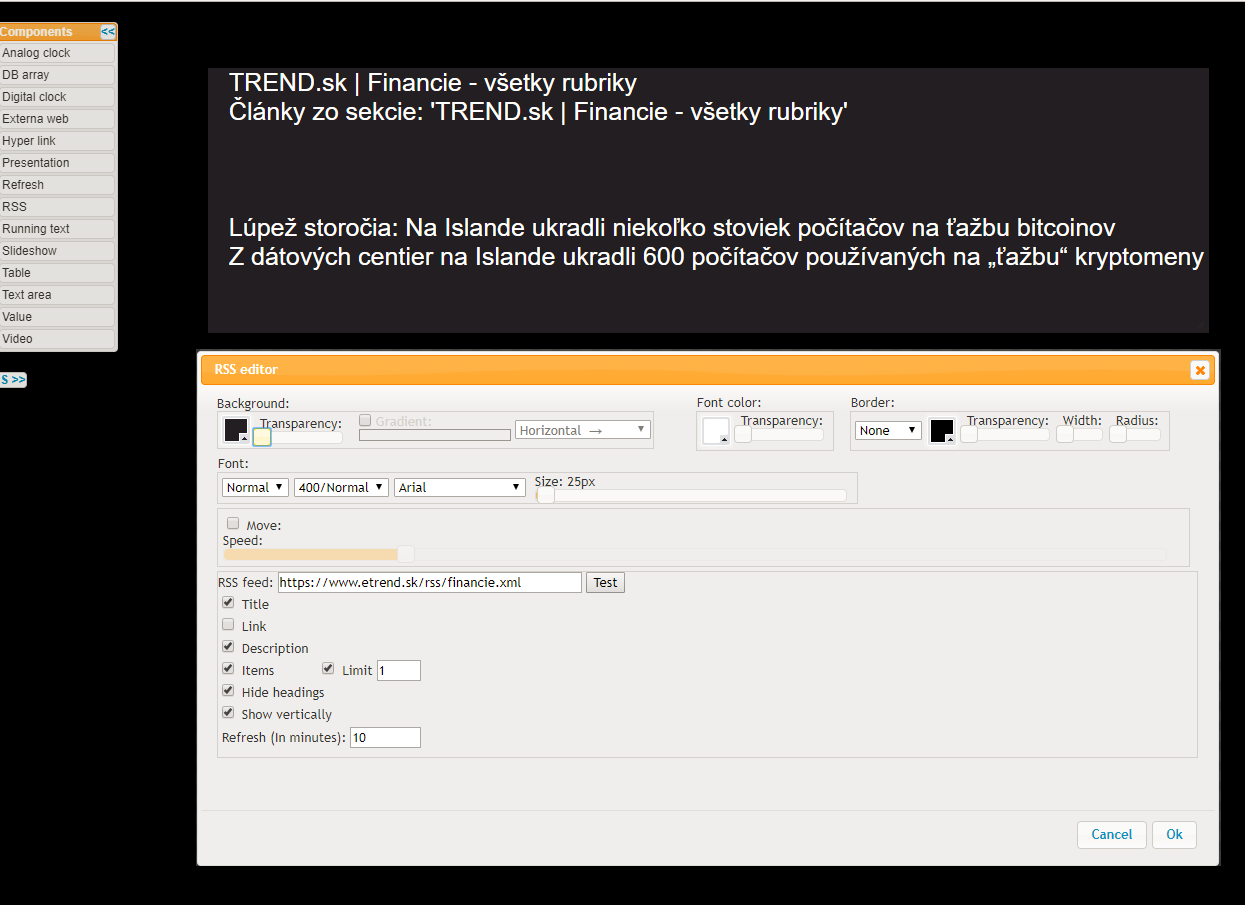
\includegraphics[width=0.95\textwidth]{RSS}
    \caption{Ukážka editora a RSS obsahu}
    \label{fig:rsseditor}
\end{figure}

\subsection{Pridanie používateľských rolí}
\textit{Časová náročnosť:} 3 dni\\
\textit{Zadanie:}\\
Zvýšiť bezpečnosť chodu aplikácie pridaním používateľských rolí a overiť ich funkčnosť:
\begin{enumerate}
\item \textbf{Administrátor} - má možnosť pridať/editovať/vymazať panel, má možnosť pridať/editovať/vymazať stránku, má prístup k nastaveniam, môže manipulovať s časovou osou.
\item \textbf{Autor} - má možnosť pridať/editovať panel, nemôže vymazať žiadny panel, má možnosť pridať/editovať/vymazať stránku, nemá prístup k nastaveniam, môže manipulovať s časovou osou.
\item \textbf{Bežný používateľ} - nemá možnosť pridať/editovať/vymazať panel, nemá možnosť pridať/editovať/vymazať stránku, nemá prístup k nastaveniam, nemôže manipulovať s časovou osou.
\end{enumerate}
\textit{Analýza:}\\
Táto požiadavka prišla od zákazníka, ktorý chcel takýmto spôsobom zvýšiť bezpečnosť chodu aplíkácie.
V prvej časti bolo potrebné upraviť tabuľku \textit{[dbo.users]} a pridať do nej stĺpec, ktorý nám bude vyjadrovať konkrétnu používateľskú rolu. V ďalšej časti, bolo potrebné prejsť všetky stránky a kontrolery a upraviť ich podľa zadania. 
\\\textit{Riešenie:}\\
Postup je rozdelený do viacerých krokov. V prvom kroku bolo potrebné upraviť databázový model, kód a  pridať stĺpec do databázy. V projekte je použitý ORM nástroj Entity framework s \textit{model-first} prístupom. Ten spočíva z použitia  modelovacieho nástroja, v ktorom je možné vizuálne pridávať entity, relácie a vytvára vzťahy medzi nimi. Tieto zmeny je následné nutné rozdielovým skriptom spustiť nad databázou. Na začiatok som sa rozhodol do projektu pridať číselník \textit{UserRoles}, ktorý bude obsahovať  názvy rolí s číslom. Ďalej som si v modeli našiel tabuľku Users, ktorá mala niekoľko stĺpcov.  Ku nim som pridal stĺpec \textit{UserRole} s typom \textit{Int32}. Aj napriek tomu, že v databáze je rola uložená ako číslo, Entity framework ju dokáže namapovať priamo do~vytvoreného číselníka. V ďalšom kroku bolo potrebné vytvoriť rozdielový skript, ktorým zmeny premietneme do databázy.
\begin{lstlisting}[language=SQL,caption=SQL skript pre pridanie používateľelskej role,captionpos=b]
						       ALTER TABLE [dbo.Users]
						       ADD UserRole int NOT NULL DEFAULT(1)
						       GO
\end{lstlisting}

V tomto prípade sme zo všetkých používateľov spravili administrátorov. Postupne som prešiel jednotlivé záznamy v databáze a upravil skupinu podľa konkrétnych používateľov. Pri vytvárani nových používateľov má administrátor odteraz možnosť zvoliť skupinu novému používateľovi.\\ Ďalšou časťou bolo prejsť všetky stránky a upraviť  niektoré časti kódu podľa skupiny prihláseného používateľa. Mojim riešením bolo do každého modelu, ktorý sa vytvára v kontroleri a zobrazuje na stránke, pridať ďalšiu premennú, ktorú naplním používateľovou skupinou. Tú dokážem zistiť vytiahnutím aktuálne prihláseného používateľa z triedy \textit{DBContextu}. \textit{DBContext} je brána, ktorá slúží na prístup a prácu s databázou. Na jednotlivých sránkach pomocou naplneného modelu  a razora vieme definovať, čo sa má ktorému používateľovi zobrazovať a čo nie. Operácie ako upravovanie a vymazávanie môže robiť iba administrátor, v našom prípade používateľská rola 1. 
%%\lstset{language=HTML5}
\begin{lstlisting}[language=html,caption=Zobrazenie operácii pre administrátora,captionpos=b]
<div class="buttonsPanel">
    @if(model.userRole == 1) {
    <div class="editedButtons">
        <img class="edit" src="@Url.Content("~/Content/Images/edit.png ")"
        onclick="boardmanage('@(b.Id)')" title="@Locale.GetLocaleString("edit")" />
        
        <img class="delete" src="@Url.Content("~/Content/Images/remove.png")"
         onclick="deleteBoard(@(b.Id))" title="@Locale.GetLocaleString("delete")"/>
    </div>
    }
</div>
\end{lstlisting}
%\subsection*{Import udalosti do databázy}
%\textit{Zadanie:}\\
%Pridať možnosť importu udalostí priamo do databázy z xlsx súboru. Pridať  chybové hlásenia pri  nesprávnom formáte dokumentu a informovať používateľa o výsledku importu
%\\\textit{Analýza}\\
%Pri niektorých zakazníkoch sme sa streli so zaujímavou požiadavkou. Pre rýchlejšie vkladanie  udalostí na jednotlivé panely by privítali možnosť nadefinovať si ich   v tabuľkovom editore (napr. Excel) a jednoduchým spôsobom vložiť do systému. Takéto riešenie ušetrí veľa času používateľa obzvlášť pri vysokých počtoch stránok a udalostí. Zároveň pridáva možnosť  do budúcnosti vytvoriť aj export udalostí, čo by znamenalo  jednoduchý a rýchly presun z jedného systému do druhého bez zásahu administrátora alebo manuálneho vytvárania.
%\\\textit{Riešenie}\\
\section{LightNet TK}
Na projekte LightNet TK som pracoval dokopy približne  30 dní. V tejto dobe  je zahrnutých aj 5 dní učenia frameworku Angular. Jednalo sa najmä o konečnú a finálnu úpravu produktu podľa potrieb zákazníka. Moja práca spočívala v úprave a vytváraní  komponentov napísaných v~Typescripte a v malej miere aj práca na API  v jazyku Java s použitím technológie Spring Boot. Vďaka použitiu material design aplikácia vyzerá moderne a prehľadne.
\subsection{Pridanie šablón pre merania na rozvádzačoch }
\textit{Časová náročnosť:} 10 dni\\
\textit{Zadanie:}\\
Pridať do projektu grafy  z meraní. Pridať možnosť zobraziť/schovať jednotlivé inštancie  z meraní. Konečný stav môže používateľ uložiť ako šablónu.
\\\textit{Analýza:}\\
Na stránke meraní sa nachádzajú 4 grafy  a vysoký počet inštancii v samotných grafoch, čo  je pre bežného úžívateľa pomerne zložité na rýchlu orientáciu. 
Šablóna bude uľahčovať zobrazenie grafov, ale najmä zprehľadní celú stránku od  údajov, ktoré používateľ nepotrebuje. Táto úloha sa bude riešiť v prezenčnej vrstve - zobrazenie použivateľovi, tlačidlo na pridanie a výber šablóny. Ukladanie jednotlivých šablón bude prebiehať  na serveri, do Postgre SQL databázy.
\newpage
\textit{Riešenie:}\\
\textbf{Klientská časť}\\
Prvým krokom bolo vymyslieť rozmiestnenie jednotlivých  tlačidiel na stránke a realizovať samotný výber šablón. To som realizoval pomocou klasického selectlistu. V angulare môžeme tento  prvok nájsť pod názvom 
\textit{<mat-select>}. V selectliste budu zobrazené šablóny stiahnuté zo servera. Pre~obmedzené miesto vo widgete grafov som sa rozhodol umiestniť tlačidlo na pridanie šablóny priamo do selectlistu. Po výbere tejto možnosti sa zobrazí dialóg pre zadanie názvu šablóny. Tento dialog je realizovaný ako samotný komponent s názvom 
\textit{MatDialog}. Po zadaní názvu sa kontroluje, či používateľ nezadal nebezpečné symboly ako úvodzovky, pomlčky, medzeru  a~podobne. V tomto zozname tiež bude možnosť zobraziť všetky grafy a inštancie bez možnosti editácie. To je vhodné vtedy, ak používatel chce mať pri vstupe na stránku zobrazené všetky údaje.  Na~grafy a zobrazenie časovej osi som použil framework \textit{vis.js}, ktorý podporuje rôzne druhy grafov a~obsahuje časovú os. Medzi ďalšie dôvody patrili, že je zadarmo, jednoducho sa s~ním pracuje a~má rozsiahlu dokumentáciu.  Ešte pred načítaním grafov sa  najskôr zo servera načítajú všetky šablóny aktuálneho používateľa. V databáze je uložená aj informácia, ktorú šablónu má používateľ predvolenú. Vďaka tomu sa zobrazia iba grafy a inštancie, ktoré používateľ zvolil. Pri zmene šablóny je znovu potrebné načítať dáta do grafov a uvolniť pamäť od~nepotrebných dát. Takisto bolo potrebné detekovať vypnutie nejakej inštancie grafu. Na obidve tieto udalosti som si implementoval eventlistener, ktorý je zabudovaný v angulari. Vďaka tomu je možné pri~zmene zavolať ľubovolnú metódu. 
\begin{lstlisting}[language=Javascript,showstringspaces=false,label=angular1,caption=Selectlist pre zvolenie šablóny s využitím nástrojov angularu,captionpos=b]
 <mat-select placeholder="{{'measurement_filter' | translate}}"
  [@SelectTemplateAnimation]='selectTemplateState' (change)="templateChanged()"
  [(ngModel)]="selectedTemplate" name="template" class="select-group-dropdown">
           <mat-option *ngFor="let template of templates " [value]="template">               
           </mat-option>
 </mat-select>
\end{lstlisting}

V ukážke \ref{angular1} možeme vidieť použité viaceré nástroje angularu, ktoré som počas celého vývoja používal. Medzi tie základné patria:
\begin{enumerate}
\item \textbf{Two-way databinding} - S touto možnosťou je možné previazať model z triedy priamo~do~HTML kódu. Ako názov napovedá zmeny sú obojsmerne premietnuté z HTML do~modelu a naopak. V našej ukážke ho využívame v \lstset{language=Javascript}
\lstinline! [(ngModel)]="selectedTemplate"! Premenná \textit{selectedTemplate} obsahuje pole objektov, ktoré sa skladajú z ID a názvu šablóny.
\item \textbf{Event binding} - Vďaka tomuto nástroju vieme pri udalosti priamo v HTML elemente zavolať metódu v triede komponentu. V našom prípade som sa rozhodol pri zmene šablóny (\textit{udalosť} \lstinline![(change)]!) zavolať metódu 
\lstinline!templateChanged()!,  ktorá inicializuje grafy  a inštancie, ktoré sú zadefinované v šablóne.
\item \textbf{String interpolation} - Tento nástroj umožnuje premietnuť  veci z triedy komponentu do obyčajného textu. Takto je možné vypísať napríklad hodnotu premennej alebo rôzny iný text. V ukážke %%\lstset{language=Javascript}
\lstinline
[showstringspaces=false]!placeholder="{{'measurement_filter' | translate}}")! využívam string interpolation na nastavenie našeptávacieho textu. Je tu tiež použitý  tzv. piping (\textit{znak '|'}), ktorý sa používa na ďalšiu modifikáciu textu, napríklad zaokrúhlenie čísiel, formát dátumu, zmena textu na veľké/malé písmena a podobne. V tomto prípade  som piping použil na preklad textu, o ktorom bližšie popisujem v ďalšej kapitole.
\end{enumerate}
\textbf{Serverová časť}\\
Pri zmenách šablón bolo potrebné tieto zmeny uložiť aj do databázy. Komunikácia so serverom  prebieha  pomocou REST API. Serverová časť je napísaná v Jave technológiou Spring boot s~použitím MVC architektúry. Vďaka tomu ostávalo  iba implementovať model a kontrolér, na~ktorý sa budem z klientskej časti dotazovať. Bolo potrebné vytvoriť metódy v kontroleri na~pridanie a vymazanie šablóny. Celý komponent som  na konci otestoval s rôznymi použivatelskými účtami pre overenie funkčnosti.
\begin{figure}[h]
    \centering
    \includegraphics[width=1\textwidth]{graphs}
    \caption{Výsledná stránka meraní }
    \label{fig:graphs}
\end{figure}

\subsection{Lokalizácia SK/EN}
\textit{Časová náročnosť:} 4 dni\\
\textit{Zadanie:}\\
Lokalizovať aplikáciu do SK/EN jazyka s možnosťou výberu jazyka.
\\\textit{Analýza:}\\
Jednou z  úloh  lokalizácie bolo určiť, či sa bude vykonávať na serveri, alebo na strane klienta. Z~dostupných riešení lokalizácie v rámci technológii Spring boot a Angular  som sa rozhodol riešiť jazykovú lokalizáciu na strane klienta, v javascripte pomocou knižnice \textit{i18n}\cite{i18n}
\\\textit{Riešenie:}\\
Použitie knižnice \textit{i18n} vo frameworku angular je pomerne jednoduché a nenáročné na použitie. Pomocou nástroja \textit{npm} si najprv nainštalujeme do projektu knižnicu.
\begin{lstlisting}[language=javascript,showstringspaces=false]
			             	         npm install i18n --save
\end{lstlisting}
Po inštalácii knižnice a  prečítaní dokumentácie  bolo  potrebné vytvoriť súbory, ktoré budú obsahovať preložené reťazce vo formáte \textit{"kľúč"}: \textit{"hodnota"}. Tieto súbory sa  musia volať podľa skratky jazyka. V mojom prípade som si v koreňovom adresári projektu vytvoril súbor \textit{sk.json} a \textit{en.json} V ďalšom kroku  bolo úlohou nájsť všetky reťazce pridať ich do  týchto súborov  aj  s preloženou hodnotou. Aby knižnica vedela, ktoré  veci sa majú prekladať je  použitý tzy. \textit{piping}, s ktorým je možné meniť a upravovať textové hodnoty v HTML kóde.
%%\lstset{language=HTML5}
\begin{lstlisting}[language=Javascript, showstringspaces=false,caption= String interpolation s použitím pipingu na preklad,captionpos=b]
		  		        {{"EmailIsNotInCorrectFormat" | translate}}"
\end{lstlisting}
Knižnica sa štandardne snaží použiť jazyk, ktorý je nastavený v prehliadači. Ak sa taký jazyk  medzi vytvorenými súbormi nenachádza, ostáva ponechaná pôvodný nepreložený kľúč. Toto správanie knižnice  nevyhovovalo z viacerých dôvodov. Ku aplikácii často pristupujú aj ľudia z iných štátov a mohlo by sa ľahko stať, že sa aplikácia vôbec nepreloží, pretože neexistuje ekvivalentná jazyková verzia. Ja som sa rozhodol  nastaviť predvolený anglický jazyk a až potom podľa jazyka prehliadača  nastaviť  prípadne slovenský jazyk. Kedže knižnica je implementovaná v angulari ako služba, bolo jednoduché k nej prístúpiť v konštruktore koreňového komponentu a nastaviť jazyk. V konštruktore bolo  tiež potrebné registrovať jazykové verzie pomocou funkcie 
\textit{addLangs()}, ktorá berie ako parameter pole názvov jazykových verzii.
\begin{lstlisting}[language=Javascript,showstringspaces=false, caption=Nastavenie jazyka v konštruktore,captionpos=b]
constructor( private translateSevice: TranslateService ) {
    console.log("App created");
	
    this.translateSevice.addLangs(['en', 'sk']);
    this.translateSevice.setDefaultLang('en');
	
    let browserLang = this.translateSevice.getBrowserLang();
    this.translateSevice.use(browserLang.match(/en|sk/) ? browserLang : 'en');
}
\end{lstlisting}
Samostatnou kapitolou bola sránka alarmov. Alarmy predstavujú  rôzne chyby, ktoré nastali pri manipulácii s osvetlením. Každý alarm má svoj chybový kód a  chybovú správu uloženú v~databáze. Úlohou bolo  pridať stĺpec ku tabuľke alarmov  s chybovou  správou v anglickom jazyku. Pri získavaní údajov zo servera sa prenášajú   verzie v obidvoch jazykoch. Pri načítani stránky s alarmami sa vyberie tá verzia, ktorá je nastavená v službe \textit{translateService}. Na zmenu jazyka počas behu aplikácie som do naviačnej lišty pridal  selectlist, ktorý  pri zmene volaním metódy \textit{setLang()} nastaví zvolený jazyk.
\subsection{Pridanie kontaktného formuláru }
\textit{Časová náročnosť:} 3 dni\\
\textit{Zadanie:}\\
Pridať komponent pre kontaktný formulár. Vytvoriť emailové konto a správne ho nakonfigurovať v aplikácii.
\\\textit{Analýza:}\\
Táto úloha sa dala rozdeliť do 2 samostatných úloh. Jednalo sa o vytvorenie formuláru, ktorý vidí používateľ a samostatné odoslanie emailu z klienta na adresu zadanú zákazníkom. Aby aplikácia bola schopná posielať emaily, bolo potrebné vytvoriť emailový účet a správne ho nakonfigurovať. Po skončení bolo potrebné overiť funkčnosť posielania na testovacie emaily.
\\\textit{Riešenie:}\\
Samostatný formulár sa skladá zo 6 polí (Meno odosielateľa, Spoločnosť, Adresa, Telefón, Email a Text správy). Tieto polia boli vyžiadané zakazníkom, pričom povinne vyplnené polia musia byť Meno, Email a Text správy. V angulári som si vytvoril triedu \textit{EmailMessageModel}, ktorá obsahovala všetky polia formuláru. Anglular obsahuje aj knižnice a nástroje na prácu s formulármi a~ich validaciu. Túto knižnicu som si musel naimportovať z  \textit{'@angular/forms'}. Pomocou two-way databinding som načítal dáta  do inštancie tejto triedy. Potrebné validácie a pravidlá sa dajú riešiť dvomi spôsobmi:
\begin{enumerate}
\item\textbf{Template-driven validácia} - do HTML časti  sa integrujú  atribúty pre validáciu vstupných polí napr.: \textit{required, minlenght, maxlenght}. Takýmto spôsobom nie je možné formulár validovať dynamicky, čo v našom prípade ani nepotrebujeme,
\item\textbf{Reactive form validácia} - pod týmto názvom sa skrýva komplexnejšia  validácia, ktorá sa používa v angular kniťnici. Validácia sa vytvára priamo v triede komponentu pomocou individuálnych metód. Toto je vhodné, ak chceme validovať nejaké polia dynamicky, napríklad kontrolovať, či  zadaná emailová adresa  už nieje použitá bez odoslania formuláru.

\end{enumerate}
 V tejto úlohe som sa rozhodol použiť \textit{Template-driven} validáciu, lebo postačuje pre náš  formulár. Pri chybe vo validácii   bolo potrebné nastaviť tlačidlo na \textit{disabled} aby sa predišlo odoslaniu chybného formuláru. 
 Druhou časťou bolo nájsť možnosť, ako posielať správy na email zakazníka. Bolo potrebné vytvoriť prostredníka, ktorý údaje z formuláru prepošle na email.  Ja som sa rozhodol vytvoriť emailovú schránku a nakonfigurovať ju v serverovej časti. Na strane servera som si vytvoril nový kontrolér s názvom  \textit{EmailController} s jedinou metódou \textit{SendEmail(EmailMessageModel message}, ktorá prijma model správy definovaný  triedou \textit{EmailMessageModel}. Posielanie správ som skúšal najskôr na firemných emailoch a po  skončení testov som v konfiguračnom súbore \textit{app.json} nastavil emailovú adresu zadanú zákazníkom.
\begin{figure}[H]
    \centering
    \includegraphics[width=0.9\textwidth]{contact}
    \caption{Kontaktný formulár s aktívnou validáciou }
    \label{fig:contactform}
\end{figure}
\subsection{Optimalizácia pre mobilné zariadenia}
\textit{Časová náročnosť:} 4 dni\\
\textit{Zadanie:}\\
Optimalizovať aplikáciu pre všetky mobilné zariadenia a bežne používané prehliadače.
\\\textit{Analýza:}\\
Responzivita webových stránok patrí v roku 2018 už k bežným štandardom a moderný web sa bez nej nezaobíde. Minimálne rozlíšenie, na ktoré som sa rozhodol aplikáciu optimalizovať  bolo na šírku  350px, čo zvládne väčšina súčasných mobilných telefónov.  Samotné rozloženie  informácii z aplikácie je rozdelené do tzv. widgetov čo predstavovalo okno s plávajúcou šírkou podľa obsahu. Ďalšou úlohou bude upraviť  texty aj v hornej lište, pretože obsahuje veľký počet informácii (čas, meno prihláseného používateľa, výber jazyka, odhlásenie).
\\\textit{Riešenie:}\\
Samotnú responzivitu som riešil  úpravou CSS tried pomocou \textit{@media} funkcií. Táto funkcia bola pridaná až vo verzii CSS3. V nej sa zadefinuje pomocou parametrov, či chceme zmeniť triedu keď je rozlíšenie väčšie alebo menšie ako zadané v parametri. Ja som sa rozhodol upravovať triedy pre 3 rôzne rozlíšenia:
\begin{enumerate}
\item \textbf{350px - 600px} - rozlíšenie, ktoré je možné nájsť na väčšine mobilných telefónov,
\item \textbf{601px - 960px} -  rozlíšenie, ktoré sa používa na tabletoch, poprípade na mobilných telefónoch otočených horizontálne (na šírku),
\item \textbf{960px a viac} -  rozlíšenie použité na notebokoch a stolových počítačoch. Na tejto sekcii bolo vykonaných najmenej úprav, keďže stránka bola vyvíjaná na notebooku s takýmto rozlíšením.
\end{enumerate}
Responzivitu môžeme jednoducho simulovať použitím vývojárskych nástrojov  v prehliadači Google Chrome. takýmto spôsobom som sa rozhodol používať 3 rôzne rozlíšenia z  definovaných rozsahov. Vo väčšine komponentov bolo potrebné pri malom rozlíšení zmeniť veľkosť z pixelov na~percentuálnu hodnotu. Tým sa dosiahol efekt, že  sú čítatelné všetky texty v závislosti od~šírky stránky a nič podstatné nieje skryté. Ďalším krokom bolo  pridať rozbalovacie menu. Pri malom rozlíšení sa stávalo, že údaje, ktoré boli v hornej lište  sa  do širky stránky nezmestili. Rozhodol som sa pridať ďalší kontajner, v ktorom bude zobrazené meno prihláseného používateľa a tlačidlo na odhlásenie. Tomuto kontajneru som priradil triedu, ktorú  pomocou selektoru nastavujem na~\textit{display:none;} alebo \textit{display:block;}
\begin{lstlisting}[language=html5,showstringspaces=false, caption= CSS optimalizácia pre jednotlivé rozlíšenia,captionpos=b]
@media only screen and (max-width: 600px) {
	.fullMenu {
        display: none;
    }
	.container {
        width: 100%;
    }
}
@media only screen and (max-width: 959px) {
    .fullMenu {
        display: none;
    }
}
@media only screen and (min-width: 960px) {
    .smallMenu {
        display: none;
    }
}
\end{lstlisting}
\begin{figure}[H]
    \centering
    \includegraphics[width=1\textwidth]{responseCompare}
    \caption{Ukážka responzivity: Neoptimalizovaná aplikácia (vľavo) a oprimalizovaná aplikácia (vpravo) }
    \label{fig:responseCompare}
\end{figure}
Okrem úpravy CSS tried bolo potrebné na mobiloch skryť aj  bočný panel s  odkazmi na mestá a rozvádzače. To som  implementoval v konštruktore hlavného komponenta  aplikácie. Ten sa vždy zavolá pri spustení aplikácie. Keďže bočný panel je komponent tretej strany, obsahuje  pomerne širokú škálu  funkcionality. Jednou z nich bolo aj funkcia \textit{hide()}. V konštruktore  stačilo detekovať šírku stránky pomocou \textit{window.width} Ak bola menšia ako  hodnota pre mobilný telefón (v našom prípade 600px) tak stačilo funkciu \textit{hide()} zavolať nad panelom. To nám zabezpečilo, že aj  pri vstupe do aplikácie bude bočný zoznam implicitne schovaný. Na záver ostávalo pridať do navigačnej lišty malú ikonu namiesto celých tlačidiel pri najmenšom rozlíšení. Po kliknuti na ikonu sa zobrazí zoznam pôvodných tlačidiel. Takto optimalizovanú aplikáciu som skúšal po~nasadení na viacerých telefónoch s viacerými prehliadačmi. Vďaka tejto úlohe som si rozšíril  svoje zručnosti v budovaní frontendu a  detailingu stránky, ktoré posúvajú celú aplikáciu zase o~level vyššie.
\newpage
\subsection{Inteligentná lišta }
\textit{Časová náročnosť:} 4 dni\\
\textit{Zadanie:}\\
Pridať navigačnú lištu s tlačidlami a aktuálnym časom. Lišta sa po posune stránky nadol skryje a po posune stránky hore sa opäť zobrazí.
\\\textit{Analýza:}\\
Inteligentnú lištu môžeme nájsť na takmer každej modernej webovej stránke. Jej úlohou je najmä zväčšiť plochu užitočných informácii na stránke, ale stále mať k dispozicii dôležité odkazy a tlačidlá  bez  zbytočného rolovania na vrch stránky. Veľký rozdiel je sporozovatelný najmä pri~prehliadaní stránky na mobilnom zariadení s malým rozlíšením. 
\\\textit{Riešenie:}\\
Pre túto úlohu bolo potrebné upraviť komponent \textit{<mat-toolbar>}. Nakoľko originálny komponent neposkytuje možnosť samoschovávania lišty, bolo potrebné ju naimplementovať. Pre úpravu komponentu bolo potrebné vytvoriť triedu v kaskádových štýlch, ktorú komponentu priradím. Zároveň bolo potrebné detekovať používateľov pohyb na stránke nahor a nadol pre zobrazenie a skrytie lišty. Pohyb  používateľa na stránke som urobil pomocou registrácie listenera priamo v hlavnom komponente.  Pre krajší efekt a lepší UX  zážitok  som okrem posunu lišty a jej skrytia pridal do~triedy  atribút na zníženie priehľadnosti (\textit{opacity:0;}). Výsledkom je  lišta, ktorá sa plynulo schová po rolovaní stránky nadol. 

\begin{lstlisting}[language=Javascript,showstringspaces=false, caption= Funkcia na odchytávanie rolovania stránky,captionpos=b]
export class ScrolllistenerDirective implements AfterViewInit {
  @Output() scrolledUp: EventEmitter<any> = new EventEmitter();
  @Output() scrolledDown: EventEmitter<any> = new EventEmitter();
  public scrollEvent: Subject<any> = new Subject();
  private currentScroll = 0;

  @HostListener('scroll', ['$event'])
  onScroll(e) {
    let el = e.target;
    let value = e.target.scrollTop;
    if (value > this.currentScroll) {
      this.scrolledDown.emit();
      this.scrollEvent.next("scrolledDown");
    }
    else if (value < this.currentScroll) {
      this.scrolledUp.emit();
      this.scrollEvent.next("scrolledUp");
    }
    this.currentScroll = value;
  }
\end{lstlisting}

\section{Správa evidencie operátorov - OAC}
Správa evidencie operátorov - OAC  je jeden z prvých projektov, ktorý beží na novej propietárne vyvinutej platforme firmy M2M solutions s.r.o. Súčasne s jej vznikom prebiehalo aj odlaďovanie chýb  a implementácia nových vecí v platforme. Jedná sa o ASP.NET webové stránky napísané v~jazyku C\#. Ako ORM nástroj  bol použitý Entity framework s prístupom code-first. Vďaka tomu je možné riadiť verziu  databázy pomocou migrácii, ktoré sa píšu priamo v C\# kóde. Projekt je vyvíjaný podľa architektúry MVC, ktorá oddeluje rôzne vrstvy systému. Súčasne s~MVC architektúrou boli použité aj mnohé ďalšie návrhové vzory. 

\begin{figure}[H]
    \centering
    \includegraphics[width=0.95\textwidth]{oacdiagram}
    \caption{Databázový model projektu Správa evidencie operátorov OAC}
    \label{fig:oacdiagram}
\end{figure}
\subsection{Platforma - Property  comparator}\label{sssec:num1}
\textit{Časová náročnosť:} 8 dni\\
\textit{Zadanie:}\\
Vytvoriť atribút na porovnávanie rôznych propert v rámci jedného modelu.
\\\textit{Analýza:}\\
Medzi väčšie  úlohy, ktoré  bolo potrebné implementovať na platforme bolo vytvorenie atribútu pre porovnávanie polí vo formulári. Táto úloha nie je  závislá iba na projekte, ale  jej využitie sa môže hodiť aj na iných projektoch, ktoré budú fungovať s týmto platformovým jadrom. V~MVC architekrúre sa validácia implementuje priamo v modeli pomocou rôznych validačných atribútov. Napríklad či je pole povinné, alebo nie, minimálna alebo maximálna dĺžka reťazca, alebo číselný rozsah. Pre zníženie záťaže servera je možné povoliť aj klientskú validáciu. Vtedy sa formulár overuje priamo v prehliadači. Ak formulár nieje  validný, na server sa neodošle a tým pádom ho server nemusí ďalej spracovávať. Validácii na serveri sa ale nemôžeme úplne vypnúť, pretože klient  má plnú kontrolu nad kódom v javascripte. Po úprave kódu môže obísť validáciu poslať aj formulár, ktorý nie je validný. V projekte je tým pádom použitá dvojitá validácia. Pod zadaním úlohy sa rozumie vytvoriť atribút, ktorý sa bude správať takisto ako validátor polí. Takáto implementácia nie je obsiahnutá v štandardnej ASP.NET knižnici, a preto ju bolo potrebné vytvoriť. Vo validátore bude potrebné prijmať názov druhého poľa, ku ktorému bude porovnávaný a operátor porovnávania. Takýmto komparátorom je možné overovať rôzne hodnoty rovnakého typu, ktoré ale musia implementovať rozhranie \textit{IComparable}. Toto rozhranie štandardne implementujú všetky jednoduché dátové typy v .NET vrátane rôznych triednych typov ako \textit{String}, \textit{DateTime}, \textit{TimeSpan} a rôzne iné.  Vďaka tomuto validátoru bude jednoduché overovať hodnoty medzi sebou, napríklad začiatok musí byť menší ako koniec, alebo hodnota v~jednom poli musí byť menšia ako v druhom poli a podobne. Súčasne bude potrebné implementovať validáciu aj na strane klienta, aby sa  formulár s nesprávnymi dátami zbytočne neposielal na server, ale vyhodnocoval priamo  na strane klienta v prehliadači.
\\\textit{Riešenie:}\\
Na začiatok som si vytvoril triedu, ktorá dedí z triedy \textit{ValidationAttribute} a implmenetuje rozhranie \textit{IClientValidatable}. Nad samotnou triedou je potrebné zadefinovať atribút \textit{[AttributeUsage]}, aby bolo jasné nad akým typom sa tento vytvorený atribút môže používať. V platforme potrebujeme porovnávať iba hodnoty vrámci jednej triedy (modelu). Práve preto som nastavil nad triedu atribút \textit{[AttributeUsage(AttributeTargets.Property)]}. Trieda musí implementovať rozhranie \textit{IComparable}, pretože iné hodnoty nie je možné implicitne bez dodatočnej logiky porovnávať. Všetky metódy rozhrania  je potrebné prepísať vlastnou funkcionalitou.  V prvom kroku  treba vytvoriť validáciu na strane servera a potom aj na strane klienta. V konštruktore atribútu nie je možné dať ako parameter inú propertu. Súčasne so vznikom atribútu však vieme zistiť v ktorej triede sa validátor práve aplikuje. Tak vieme zistiť jej názov, typ a pristupovať  k jednotlivým propertám daného modelu. Ja som sa kvôli jednoduchosti rozhodol v parametri poslať reťazec s názvom druhej property.  Pre prípad, keď by sa náhodou premenovala,  kompilátor by nehlásil žiadnu chybu, pretože ju berie ao reťazec. Toto môžeme vyriešiť náhradou reťazca príkazom  \textit{nameof(<propertyName>)}. Tym zaručíme, že aj ked sa  náhodou premenuje, komplikátor nám okamžite podčiarkne chybu, lebo taký názov nepozná. V parametroch bolo potrebné ďalej zadať operátor, pre aký sa ma vyhodnocovať validácia ako správna. To som vyriešil vytvorením číselníka s názvom \textit{CompareOperator}, ktorý obsahuje základné porovnávacie operácie (<, >, ==, <=, >=). Teraz už vieme pristupovať k propertám triedy a vieme na základe čoho ich chceme porovnávať. Samotné overovanie  validity modelu sa vykonáva až vo funkcii \textit{IsValid(object o, ValidationContext validationContext)}. Najskôr som musel overovať, či jednotlivé property spĺňajú všetky kritéria pre porovnávanie, či sú alokované, ale aj či sú rovnakého typu. Ak  niektorá podmienka nie je splnená, je vyhodená výnimka, ktorá sa zapíše do  serverových logov. Keďže platforma  musí byť multijazyková,  bolo potrebné chybovú správu preložiť vrátane preložených názvov. ASP.NET obsahuje atribút \textit{[DisplayName]}, v ktorom je možné zadefinovať názov a súbor, v ktorom má hľadať jeho preloženú verziu. V ukážke \ref{lst:displayname} je znázornené zistenie preloženého názvu. Ak  atribút \textit{[DisplayName]} nie je definovaný, použije sa originálny názov, ktorý je zadaný v kóde ako názov property. \\
 

\begin{lstlisting}[language=Javascript,showstringspaces=false, caption= Klientská validácia - získanie preloženého mena,captionpos=b,label={lst:displayname}]
private static string GetDisplayNameForProperty(Type containerType, string propertyName)
{
    var typeDescriptor = GetTypeDescriptor(containerType);
    var property = typeDescriptor.GetProperties().Find(propertyName, true);
    if (property == null)
    {
        throw new ArgumentException
        (string.Format(CultureInfo.CurrentCulture, 
        Resources.Common_PropertyNotFound,  containerType.FullName, propertyName));
    }
    var attributes = property.Attributes.Cast<Attribute>();
    var display = attributes.OfType<DisplayAttribute>().FirstOrDefault();
    if (display != null)
    {
        return display.GetName();
    }
    var displayName=attributes.OfType<DisplayNameAttribute>().FirstOrDefault();
    if (displayName != null)
    {
        return displayName.DisplayName;
    }
    return propertyName;
}
\end{lstlisting}
Druhou časťou bolo implementovať validáciu na strane klienta. Tá pozostávala zo zostavenia údajov, ktoré sa budu spolu s modelom  prenášať do HTML stránky ako atribúty HTML komponentu. Týmto spôsobom som sa rozhodol poslať názov druhej property a jej preložený názov, operátor a preloženú chybovú správu. V javascripte som musel  vytvoriť vlastný validátor s pridanou funkcionalitou a pomocou jQuery dostať hodnoty z polí vo formulári. Najväčší problém, s ktorým som sa stretol, bolo detekovať, či je hodnota časového typu. Javascript štandardne takéto polia  vo formulároch  berie ako text, v ktorom sa nedajú porovnávať dve dátumové hodnoty. Aby som zistil, či je pole časového typu, bolo potrebné zistiť, či obsahuje triedu \textit{.time} alebo \textit{.dateTime-utc}. Ak pole obsahovalo jednu z týchto tried, previedol som ho na dátumovú hodnotu pomocou knižnice \textit{moment.js}, ktorá obsahuje funkcionalitu na porovnávanie  dátumov. Na koniec som otestoval aj klientskú validáciu. Formulár som vyplnil chybnými hodnotami a validátor ma okamžite upozornil  červenou hláškou (\textit{pozri obr. \ref{fig:propertycompare}}) bez toho, aby som formulár odoslal.
\begin{figure}[H]
    \centering
    \includegraphics[width=1\textwidth]{PropertyComparator}
    \caption{Overenie funkčnosti Property comparator s poľami typu TimeSpan}
    \label{fig:propertycompare}
\end{figure}
\newpage
\subsection{Implementácia business logiky}
\textit{Časová náročnosť:} 5 dni\\
\textit{Zadanie:}\\
Implementovať projektovú business logiku na správu pozícií a produkčných modelov.
\\\textit{Analýza:}\\
Pre oddelenie business logiky od kontrolerov a pre prácu s databázou je v projekte použitý návrhový vzor \textit{Repozitár}. V projekte je vytvorený repozitár pre každú entitu, čím  sprehľadnuje celú aplikáciu a sústreduje všetky metódy na prístup do databázy na jedno miesto v rámci entity. Ďalší  použitý návrhový vzor je \textit{Unit Of Work}. Ten bol do projektu zaintegrovaný preto, aby každú malú operáciu nebol nutný zásah do databázy. Predstavme si situáciu, keď v jednej sitácii chceme  napríklad  vymazať 50 záznamov a pridať ďalších 50 v jednej akcii. \textit{Unit of work} zabezpečuje to, že tieto zmeny sú najskôr uložené  iba v pamäti a až v závere akcie sa tieto zmeny premietnu do databázy funkciou \textit{Commit()}
Na konfiguráciu  rôzych komponentov a~služieb existuje mnoho doplnkov tretích strán. Jedným z nich je aj \textit{Autofac}, ktorý používa  nástroj \textit{Dependency injection}. Vďaka tomu je možné pomocou rozhrania a  implementácie zadefinovať množinu komponentov, ktoré sa použijú v projekte. Pomocou \textit{Dependency injection} je jednoduché namapovať do konštruktora kontrolera akúkoľvek  komponentu, ktorú sme si vytvorili. 
\\\textit{Riešenie:}\\
V tomto projekte sa \textit{Autofac} používa napríklad pre na vkladanie  komponenty \textit{Logger}. \textit{Logger} má na starosti vytvárať rôzne systémové udalosti a informuje o  práci v aplikácii ako pridanie, odstránenie, úprava záznamov a podobne. Okrem loggera je v kontroleri použitá aj trieda \textit{IProductionManager}, ktorá zastrešuje všetky  datábázové operácie a doménovú logiku pre každú entitu. V~tejto triede sú postupne vytvárané metódy, ktoré zase volajú metódy z \textit{IRepository}. Triedy, ktoré implementujú \textit{IRepository} už pracujú na úrovni Entity Frameworku, ktorý sa používa takmer vo väčšine projektov, ktoré bežia na ASP.NET. Postupne  som začal pridávať metódy do~rozhrania \textit{IProductionManager}, ktoré potrebujem pre  jednotlivé stránky a operácie. Na úrovni managera som si  tieto metódy implementoval a pridal im vlastnú logiku  podľa potreby. Okrem vytiahnutia záznamov z databázy bolo napríklad potrebné odstrániť záznamy, ktoré majú stĺpec \textit{Obsolete== true}. Údaj hovorí o tom, že  záznam je vymazaný. Záznamy nie sú vymazávané fyzicky, ale majú nastavený príznak  \textit{Obsolete} na \textit{true}. Tým je jednoduché zabezpečiť spätnú obnovu dát v prípade neúmyselného vymazania. Niektoré operácie si zase vyžadovali vytvorenie ďalších objektov v databáze. Jednoduchý príklad môžeme vidieť v ukážke \ref{lst:addTraining}. Okrem vytvorenia preškolenia sa musí podľa  pozícii prekolenia vytvoriť neexistujúce záznamy ľudí, ktorí  sú k~pozícii priradení. Vytvoriť sa môžu iba ak majú level zatrénovanosti väčší ako 0, teda na danej pozícii už pracujú dlhšie. Na konci metódy musíme zavolať funkciu \textit{SaveChangesInternal()}, ktorá prenesie všetky zmeny z pamäte  priamo do databázy. Podobnú logiku bolo  potrebné zaintegrovať  pre všetky ostatné operácie s entitami. Vďaka tejto úlohe som získal  prehľad architektonických vzorov, ktoré sa používajú na oddelenie rôznych vrstiev, čím sa zvyšuje celková prehľadnosť a~efektivita celého kódu, ale aj behu aplikácie.\\\\
\begin{lstlisting}[language=Javascript,showstringspaces=false, caption= Implementácia funkcie na pridanie preškolenia,captionpos=b,label={lst:addTraining}]
public async Task CreateTrainingAsync(Training training)
{
  this.ThrowIfDisposed();
  var trainingRepository = this.UnitOfWork.GetRepository<ITrainingRepository>();
  var oeRepository = this.UnitOfWork.GetRepository<IOperatorExperienceRepository>();
  var posRepository = this.UnitOfWork.GetRepository<IPositionRepository>();

  var posIds = training.Positions
  			   .Select(p => p.Id)
  			   .ToArray();
  var allOEList = await oeRepository
  		           .GetAllOperatorExperiencesByPositionListAsync(posIds);
  var operatorUserNames = allOEList
  			   .Where(oe => oe.Level > 0)
  			   .Select(oe => oe.Operator)
  			   .Distinct();
  var trainers = training.Trainers
  			   .Select(tr => tr.Trainer);
  var allTrainingOperators = operatorUserNames
  			   	.Union(trainers)
  			   	.ToList();
  trainingRepository.Create(training);
  await this.CreateTrainingOperatorsAsync(training, allTrainingOperators);
  await this.SaveChangesInternal();
}
\end{lstlisting}

\subsection{Formulár na pridanie pozície}
\textit{Časová náročnosť:} 4 dni\\
\textit{Zadanie:}\\
Vytvoriť formulár na pridanie a editáciu pozícii podľa projektovej dokumentácie.
\\\textit{Analýza:}\\
Projekt sa z veľkej miery skladá z rôznych formulárov na editáciu a pridávanie  dát do databázy. Jednou z úloh, ktoré mi boli pridelené, bolo aj vytvorenie formuláru na pridanie pozície. Pozícia je entita, na ktorá  predstavuje fyzické miesto  v sklade. Mojou úlohou bude  vytvoriť model, pohľad (view) a  implementovať  metódu v kontroleri, ktorá bude dáta  spracovávať. \\
\\\textit{Riešenie:}\\
V prvom kroku, som si vytvoril model v priečinku, kde sú ostatné modely projektu. Tento model obsahuje  všetky polia, ktoré sa nachádzajú aj v entite. Nad každé pole je možné zadať rôzne atribúty. V mojom prípade som použil atribúty \textit{[Required]}, ktorý značí, že pole  musí byť vyplnené nejakou hodnotou a \textit{[MaxLength(512)]}a \textit{[MaxLength(64)]}, ktoré značia maximálny počet znakov v textovom reťazci. Okrem štandardných atribútov na validáciu bolo potrebné aj validovať  správnosť IPv4 adresy. Na to som použil regulárne výrazy, ktoré C\# štandardne podporuje. V tomto modeli sa nachádzali aj dve polia, ktoré bolo potrebné porovnať medzi sebou. Z~dokumentácie projektu vyplývalo, že pole \textit{Pracovný čas} musí byť menšie ako pole \textit{Max. pracovný čas}. Na toto sa  dá využiť platoformový \textit{Property comparator}, na ktorom som pracoval ako na samostatnej úlohe. Bližšie je o ňom  je popísané v sekcii \ref{sssec:num1}
\begin{lstlisting}[language=Javascript,showstringspaces=false, caption= Časť modelu pozície s ukážkou validačných atribútov,captionpos=b]
 public class PositionModel
 {        
        [RegularExpression(@"^((25[0-5]|2[0-4][0-9]|[01]?[0-9][0-9]?)\.)
        {3}(25[0-5]|2[0-4][0-9]|[01]?[0-9][0-9]?)$", 
        ErrorMessage ="Not valid IPv4 address")]
        [Display(Name = "IPAddress", ResourceType = typeof(PositionLocale))]
        public string IPAddress { get; set; }

        [Required]
        [M2MSComparator(CompareOperator.LESS_THAN, nameof(MaxWorkDuration))]
        [DataType("TimeSpan")]
        [Display(Name = "WorkDuration", ResourceType = typeof(PositionLocale))]
        public TimeSpan WorkDuration { get; set; }

        [Required]
        [M2MSComparator(CompareOperator.MORE_THAN, nameof(WorkDuration))]
        [DataType("TimeSpan")]
        [Display(Name = "MaxWorkDuration",ResourceType = typeof(PositionLocale))]
        public TimeSpan MaxWorkDuration { get; set; }
        
        [StringLength(512)]
        [Display(Name = "Description", ResourceType = typeof(PositionLocale))]
        [DataType(DataType.MultilineText)]
        public string Description { get; set; }        
 }
\end{lstlisting}
\section{Navigácia v budovách - analýza}
Navigácia je v sučasnosti veľmi rozsiahlou problematikou, o ktorej by sa dala napísať samotná bakalárska práca. Moderné systémy ako napríklad GPS  sú najpoužívanejšie a najznámejšie. Fungujú  na základe odozvy signálu z niekoľkých satelitov, ktoré sa voľne pohybujú vo vesmíre.  GPS systém  má však podstatnú nevýhodu - priechod signálu cez prekážku. Ak by sme chceli použiť GPS signál  napríklad v podzemí alebo v budove, signál by sme  chytili iba veľmi sporadicky, alebo dokonca vôbec. Firma, M2M solutions sa venuje najmä priemyselným riešeniam. Jednou z akvizícii bolo  aj navigovanie  a lokalizácia v priestore - najmä vo výrobných  halách a skladoch. Mojou úlohou bolo skúsiť  nájsť všetky dostupné riešenia  s krátkou analýzou. Okrem toho bolo mojou úlohou skúsiť zbierať dáta zo senzorov mobilu  a analyzovať ich, či je možné z nich získať  zmenu  pozície bez použitia GPS systému. Celá akvizícia je iba v prvej  fáze  analýzy a preto ju rozoberiem iba okrajovo. 

\subsection{Porovnanie dostupných technológii}
\textit{Časová náročnosť:} 4 dni\\
Mojou prvou úlohou bolo nájsť a  porovnať všetky dostupné technológie, ktoré  by sa potenciálne mohli použiť na navigáciu v budovách bez použitia GPS systémov. V analýze by mali byť zahrnuté  výhody, nevýhody,  technológia, analýza ceny, presnosť. Všetky informácie som čerpal z internetových zdrojov\cite{lee2007comparative} a rôznych videí. Ja som sa rozhodol o každej technológii v krátkosti popísať a najdôležitejšie informácie zhrnúť do tabuľky \ref{tabulatorka}.
\begin{itemize}
\item\textbf{Magnetické pole} - technológia je založená na  meraní úrovne magnetického poľa. Vychádza z toho, že každé miesto v budove má jedinečnú hodnotu magnetického poľa a je možne na základe tejto hodnoty určit približnu lokáciu. Tento systém je možné použiť v~budovách, kde nedochádza k  presunu nábytku a  veľkých objektov. Pre použitie v priemysle a v skladoch  s častým presúvaním rôznych kovových predmetov  a pohybom okolo silných elektromotorov je tento systém nepoužiteľný.
\item\textbf{BLE beacony} - v súčasnosti patrí jedno k najpoužívanejším  lokalizačným systémom  bez použitia GPS. Technológia pozostáva  z rozmiestnenia bluetooth zariadení po budove a~meraním útlmu signálu  napríklad mobilom. Pre zvýšenie životnosti týchto zariadení sa zvyčajne používa štandard BLE (\textit{Bluetooth Low Energy}), ktorý je v potovostnom režime a aktivuje sa iba pri požiadavke na komunikáciu. Pri  zistení úrovne signálu z  3 rôznych zariadení je možné pomocou trilaterácie\citep{trilat} vypočítať približnú polohu objektu. Zariadenie je však veľmi náročné z hľadiska počiatočnej aj dlhodobej  ceny. Pri výrobnej hale  100x100m by bolo potrebné použiť minimálne 100 bluetooth zariadení. Každé zariadenie potrebuje inštaláciu a prívod napájania, čo predstavuje vysoké náklady pre zákazníka. 
\item\textbf{Wifi} - vychádza z podobných princípov ako BLE beacony. Jediným rozdielom je to, že je možné použiť už existujúcu infraštruktúru wifi access pointov v budovách. Veľkou nevýhodou je citlivosť na prekážky a nedostatočná presnosť.
\item\textbf{UWB} - ultra wideband je novšia technológia. Bola navrhnutá pre vyriešenie problémov, ktoré vznikajú pri predchádzajúcich riešeniach. Tým, že pracuje na  vysokej frekvencii 3GHz až 10GHz, so šírkou pásma až 500MHz dokáže  bez problémov prejsť aj prekážkami a stenami bez zníženia presnosti. Výrobcovia technológie uvádzajú presnosť až 30cm, ktorá však v realite dosahuje nižšie výsledky. Medzi jej nevýhody patrí najmä vysoká cena zariadení a limitujúci maximálny počet navigovaných objektov v počte približne 10.
\item\textbf{Akcelerometer}  - na požiadanie môjho konzultanta Borisa som dostal za úlohu preskúmať  aj  možnosť využiť   senzory z mobilu ako navigáciu. Jej výhody by mali plynúť z~jednoduchosti použitia, vyhnutiu sa vybudovaniu infraštruktúry  a nulovej ceny inštalácie. Na zistovanie pohybu  je použitelný  akcelerometer. Ten zbiera údaje o zrýchlení v jednotkách \textit{m/s\textsuperscript{2}}. Podľa teórie, by sme mali byť schopní prvým integrálom vypočítať rýchlosť a druhým integrálom prejdenú vzdialenosť.
\end{itemize}

\begin{table}[htb]
\centering
\begin{tabular}{|l|c|c|c|c|c|}
\hline
                              & \textbf{Mag. pole} & \textbf{BLE beacony} & \textbf{Wifi} & \textbf{UWB}  & \textbf{Akcelerometer} \\ \hline
\textbf{Presnosť}             & 1-2.8m                        & 2m                         & 4m            & \textless30cm & Veľmi nepresné            \\ \hline
\textbf{Dosah}                & -                             & 10m                        & 15m           & 25m           & -                         \\ \hline
\textbf{Vstupná investícia}   & Veľmi nízka                   & Veľmi vysoká               & Nízka         & Veľmi vysoká  & Veľmi nízka               \\ \hline
\textbf{Cena za údržbu}       & Nízka                         & Veľmi zložitá              & Nízka         & Veľmi vysoká  & Veľmi nízka               \\ \hline
\textbf{Zložitosť inštalácie} & Nízka                         & Veľmi zložitá              & Zložitá       & Zložitá       & Žiadna                    \\ \hline
\end{tabular}
\caption{Porovnanie  jednotlivých technológií}
\label{tabulatorka}
\end{table}

\subsection{Zber dát zo senzorov  v mobile}
\textit{Časová náročnosť:} 3 dni\\
Po  analýze nasledovalo aj napriek prevyšujúcim nevýhodam úloha zbierať dáta zo senzorov v~mobile.  Jednalo sa najmä o akcelerometer, gyroskop a magnetometer. Tieto údaje mali byť  ukladané do súboru, aby sa následne z nimi mohlo manipulovať a analyzovať ich. Mojou úlohou bolo vytvoriť  aplikáciu pre android, ktorá tieto dáta bude zbierať a vymyslieť mechanizmus na ich uloženie. Senzory v android telefónoch sa správajú ako služby. Rýchlosť zberu dát je možné zadefinovať pre každý senzor zvlášť. Je možné  definovať  normálnu rýchlosť (\textit{SENSOR\_DELAY\_NORMAL}),  rýchlosť pre UI optimalizáciu, ktorá zbiera  dáta v obmedzenom režime (\textit{SENSOR\_DELAY\_UI}) a  vysokú rýchlosť zberu dát (\textit{SENSOR\_DELAY\_FASTEST}). Ja som sa rozhodol zbierať  údaje v móde \textit{SENSOR\_DELAY\_NORMAL}. Vytvoril som si  triedu, ktorá obsahuje kolekciu objektov meraných dát. Zakaždým, keď sa dáta zo senzoru ziskajú, pridajú sa do tejto kolekcie. Keď používateľ bude chcieť ukončiť zber dát, tlačidlom na obrazovke vypne aj ukladanie dát a tie sa uložia do súboru v mobilnom telefóne. Údaje sú ukladané ako obyčajný text a sú oddelené čiarkou pre jednoduché analyzovanie v rôznych programoch na prácu s~grafmi. Triedu na zber a ukladanie dát  som vytvoril ako statickú s názvom \textit{SensorDataRecorder}. Trieda obsahuje  2 metódy. Metódu na vkladanie záznamov do kolekcie  \textit{Insert(SensorData record)}  a~metódu na uloženie kolekcie do súboru v telefóne (\textit{WriteToFile() s})
\newpage
\lstset{language=Java}
\begin{lstlisting}[language=Java,showstringspaces=false, caption= Metóda na ukladanie záznamov do mobilného telefónu,captionpos=b]
public static void WriteToFile()
{
   final File path =   new File(Environment.getExternalStorageDirectory()
   + File.separator + "Logs");
   StringBuilder sb = new StringBuilder();
   for(int i =0; i< sensorDataCollection.size(); i++) {
       SensorData item = sensorDataCollection.get(i);
       sb.append(ConvertDataToString(item));
       sb.append("\n"); // add new line
   }
   String dataString = sb.toString();
	
   // Make sure the path directory exists.
   if(!path.exists())
   {
       // Create it, if it doesn't exit
       path.mkdirs();
   }
   SimpleDateFormat formatter = new SimpleDateFormat("yyyy_dd_MM__HH_mm_ss");
   Date now = new Date();
   String fileName = "LOG_" + formatter.format(now) + ".csv";
   final File file = new File(path, fileName);
   try
   {
       file.createNewFile();
       FileOutputStream fOut = new FileOutputStream(file);
       OutputStreamWriter myOutWriter = new OutputStreamWriter(fOut);
       myOutWriter.append(dataString);
       myOutWriter.close();
       fOut.flush();
       fOut.close();
       sensorDataCollection.clear();
       Log.d("SensorDataRecorder", "File write success");
   }
   catch (IOException e)
   {
       Log.e("Exception", "File write failed: " + e.toString());
   }
}
\end{lstlisting}

\subsection{Implementácia Kalmanovho filtra}
\textit{Časová náročnosť:} 4 dni\\
Po úspešnom zozbieraní dát prišla na rad ich analýza a výpočty. Hneď na začiatku bolo z grafu vidieť, že signál je značne zašumený, čo môže  výrazne ovplyvniť  výsledok. Hlavnou podstatou a požiadavkou je zistiť zmeny polohy z týchto údajov. Aby sme z akcelerácie vypočítali  zmenu pozície, je potrebné vypočítať najskôr rýchlosť prvým integrálom zo zistenej akcelerácie a zmeny času. Ako počiatočná rýchlosť \textit{v\textsubscript{0}} je na začiatku nastavená 0m/s. Po každej iterácii sa  súčasná  rýchlosť nastaví ako  počiatočná rýchlosť nasledujúcej iterácie.
\begin{equation}
v=  v_0+at 
\end{equation}
Dáta z mobilu som zbieral v rôznych režimoch. Najskôr to bola chôdza, beh, ale aj volne položenie mobilu na stole. Po analýze dát a  vyhodnotení meraní som prišiel na to, že signál je zašumený. To spôsobuje obrovskú odchýlku v rýchlosti a tým pádom aj v pozícii. Aj pri volne položenom telefóne sa zo šumu za 1 sekundu naindukoval signál, ktorý zmenil pozíciu o približne 30cm. Po~konzultácii s  ostatnými členmi v tíme sme sa rozhodli nájsť  spôsob, ako tento šum čo najviac minimalizovať. 
Na zníženie šumu zo signálu je možné použiť Kalmanov filter\cite{bishop2001introduction}, ktorý počíta hodnoty  na základe vzoriek z predchádajúcich hodnôt. Vďaka správnemu nastaveniu   filtra, je možné  šum minimalizovať bez výrazného orezania užitočného signálu a časového posunu.
\lstset{language=Java}
\begin{lstlisting}[language=Java,showstringspaces=false, caption= Metóda na spracovanie hodnoty pomocou Kalmanovho filtra,captionpos=b]
public double getFilteredValue(double measurement) {
    this.pError = this.pError + this.qNoise;

    //measurement update
    this.kGain = this.pError / (this.pError + this.rNoise);
    this.value = this.value + this.kGain * (measurement - this.value);
    this.pError = (1 - this.kGain) * this.pError;
	
    return this.value;
}
\end{lstlisting}



\begin{figure}[h]
    \centering
    \includegraphics[width=1\textwidth]{kf}
    \caption{Porovnanie hodnôt s výsledkom Kalmanovho filtra na y-os akcelerometra}
    \label{fig:kalman}
\end{figure}
\newpage	
\chapter{Záver}
\section{Využitie znalostí získaných počas štúdia}
Počas praxe som mal možnosť využiť svoje znalosti z mnohých  predmetov absolvovaných počas štúdia. Kedže som na prax nastúpil ako programátor, najviac som využil znalosti z predmetov, ktoré sa zameriavali na vývoj softvéru. Pre mňa mal veľký prínos predmet SWI, ktorý sa zaoberal návrhovými vzormi a celým procesom  vývoja softvéru od analýzy až po nasadzovanie u zákazníka a údržbu. Preto som znalosti z predmeti SWI využíval takmer na dennodennej báze. Pri práci s databázami som využil vedomosti, ktoré som sa naučil na predmete UDBS. Počas praxe som používal najmä MS SQL a vedomosti z UDBS mi úplne postačovali. Jednalo sa najmä o  výber dát z tabuliek a  úprava tabuliek. Pri vývoji android aplikácie na zber údajov mi pomohli vedomosti z predmetu TAMZ2. Vďaka tomu som už  na začiatku projektu mal všeobecný prehľad android architekrúry a vedel som vytvoriť jednoduché používateľské rozhranie. V neposledom rade mi pomohli aj  vedomosti z predmetu VIS, vďaka ktorým som vedel pochopiť mnoho návrhových  vzorov, koré sa na projektoch vo firme používajú.
\section{Chýbajúce znalosti a nové technológie}
Každá firma používa  svoje vlastné postupy a frameworky, ktoré sa v škole  nemusia učiť. Mojím najväčším nedostatkom bol javascriptový framework Angular, o ktorom som pred tým vôbec nepočul. Keďže som s týmto frameworkom pracoval  asi 5 mesiacov,  získal som základnú znalosť pre prácu s ním. Svoju ďalšiu  slabú stránku som  postrehol  aj pri analýze  na projekte \textit{Správa operátorov OAC}. Tu som si všimol, že je obrovský rozdiel z pohľadu zákazníka a programátora. Aj keď analýza bola niekoľkokrát upravovaná, až pri vývoji sa prišlo na to, že zakazník požadoval  trochu odlišnú vec ako programátor z analýzy pochopil. Preto by som privítal predmet, ktorý by sa venoval vo väčšej miere aj zbieraniu požiadaviek od zákazníka a komunikáciu. Tieto veci mi na~škole chýbali a z mojich nadobudnutých skúsenosti a postrehov sú veľmi dôležité. Jedna z~dalších vecí, ktoré mi počas praxe chýbali, bolo riadenie práce v tímoch a správa verzií produktu. Aj keď som sa s verzovacím systémom stretol napríklad na predmete TAMZ2, tieto znalosti určite neboli dostatočné a neriešili prácu viacerých ľudí súčasne na jednom projekte. Musel som sa naučiť, ako funguje rozdelovanie úloh na projekte, diskutovať výsledky práce na pravidelných denných SCRUM meetingoch. Okrem toho som si musel bližšie naštudovať aj riešenie konfliktov v repozitári, ktoré  vznikali často pri  väčšom počte ľudí na projekte.

\section{Celkové vyhodnotenie odbornej praxe}
Z môjho hľadiska  hodnotím absolvovanie praxe prínosne. Prax mi  dala možnosť zúčastniť sa  na~reálnej práci  na IT projektoch od analýzy až po nasadenie u zákaznikov, správu verzii, ale aj manažment okolo projektov. Vďaka praxi som mal možnosť pracovať v tíme s viacerými skúsenými programátormi, ktorí mi vedeli vysvetliť aj veci, ktorým som pred tým nerozumel. Na~praxi som mal možnosť vyskúšať si vedomosti a znalosti získané  počas školy, ale aj naučiť sa  veľké množstvo nových technológii ako Angular, TypeScript alebo Entity framework. Vďaka praxi som taktiež získal praktické skúsenosti, ktoré sú pre každého informatika podstatne dôležité najmä pri hľadaní pracovného miesta v IT. Keďže  dokumentácia aj analýzy od zákazníkov boli v anglickom jazyku, podarilo sa mi čiastočne vylepšiť aj úroveň angličtiny, ktorá je v IT nevyhnutnosť. Vo firme M2M Solutions s. r. o. plánujem pracovať naďalej  a rozvíjať svoje vedomosti aj počas magisterského štúdia.\\
\begin{table}[h!]
\centering
\begin{tabular}{|c | c | c | c|} 
 \hline
  & Počet hodín & Počet dní\\ [0.5ex] 
 \hline
 Infopanely & 56 & 7  \\ 
Lightnet TK & 235 & 29  \\
Správa operátorov - OAC & 150 & 19  \\
 Navigácia v budovách - analýza& 85 & 11   \\
 \hline
\end{tabular}
\label{tabHodiny}
\caption{Odpracovaný čas na jednotlivých projektoch}
\end{table}

%\backmatter

\newpage
\thispagestyle{empty}
\nocite{*}
\clearpage

\printbibliography[title={Literatúra}]

\end{document}


